\section{PNL User Interaction Mode}

The RMA system introduces three PNL user roles/responsibilities\footnote{All activities are performed in the context of the one workshop.}:

\begin{itemize}
	\item Movement Advice User -- the role where the user's concern is processing of movement advices such as placement of rotables onto and receiving off advices.
	\item Rotable Movement User -- the role where the user's concern is rotable fitment/defitment operations.
	\item Completion Certificate User -- the role where the user's concern is processing (review and acceptance) of pending Completion Certificates; this role is in development and will be added to this document later.
\end{itemize}

From the User Interface (UI) point of view, different roles are supported using a concept of the UI \emph{perspective}. Each perspective defines a set of controls that are designed specifically to support role's responsibility. The following perspective are described in this document:
\begin{itemize}
	\item Movement Advice -- the perspective for Movement Advice User.
	\item Rotable Movement -- the perspective for Rotable Movement User.
	\item All-in-One -- the perspective for advanced operations (e.g. supports direct defitment of rotables on a movement advice), which combines Movement Advice and Rotable Movement perspectives in one; 
\end{itemize}

The following sections provide a more comprehensive overview of each of the perspectives.
\clearpage

\subsection{Movement Advice Perspective}

\emph{Movement Advice Perspective} is designed to facilitate movement advice operations such as:
\begin{itemize}
  \item Movement advices creation.
  \item Placement of rotables onto a selected movement advice.
  \item Movement advice dispatch
  \item Receiving of rotables from a selected movement advice.
\end{itemize}

\hyperref[fig:01-movement-advice-perspective]{Figure~\ref*{fig:01-movement-advice-perspective}} depicts the UI specific for the Movement Advice perspective, which consists of two panels -- one for location and selection of rotables, another - for movement advice management. Rotables are moved from onto a selected movement advice with a simply drag and drop or by clicking the \emph{Add} button.

\begin{figure}[!h]
\centering
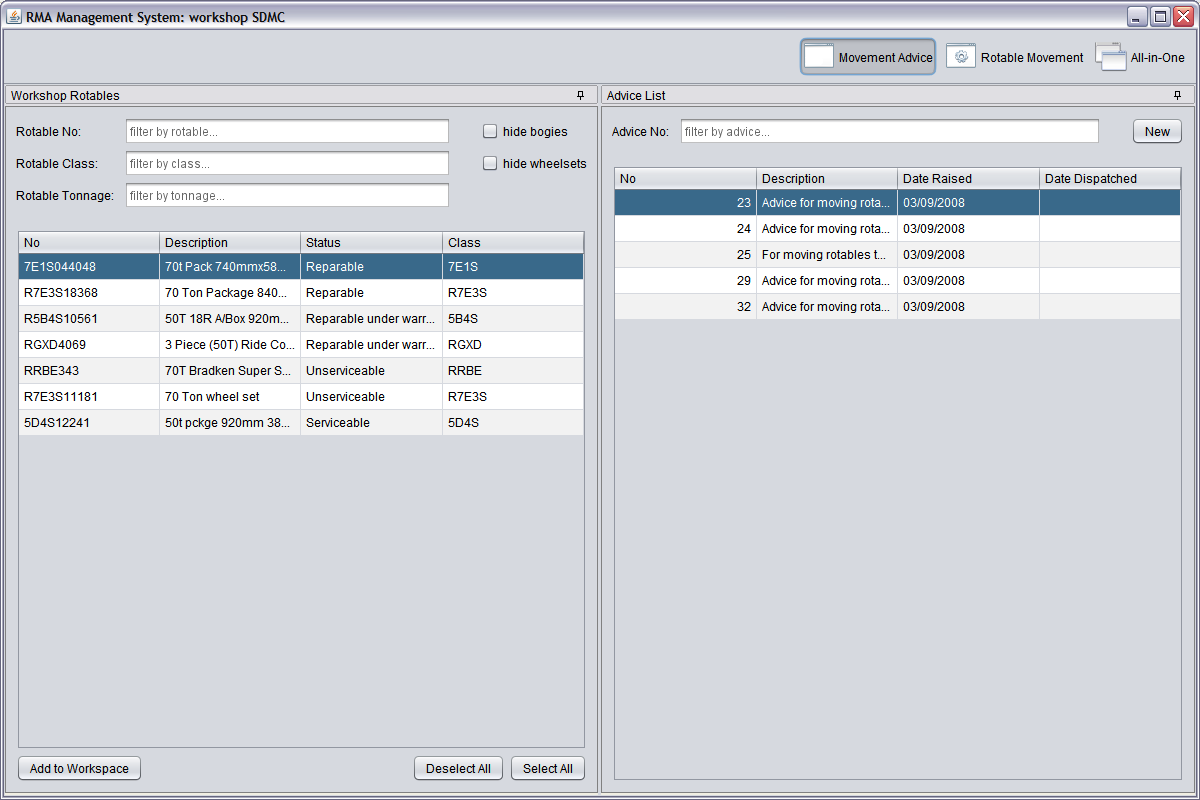
\includegraphics[scale=0.37]{chapters/02-user-interface/images/01-movement-advice-perspective.png}
\caption{Movement Advice Perspective}\label{fig:01-movement-advice-perspective}
\end{figure}

A detailed representation of the movement can be activated by selecting a corresponding row in the grid with movement advices. \hyperref[fig:01-movement-advice-perspective]{Figure~\ref*{fig:01-movement-advice-perspective}} depicts details for advice number 23.

\begin{figure}[!h]
\centering
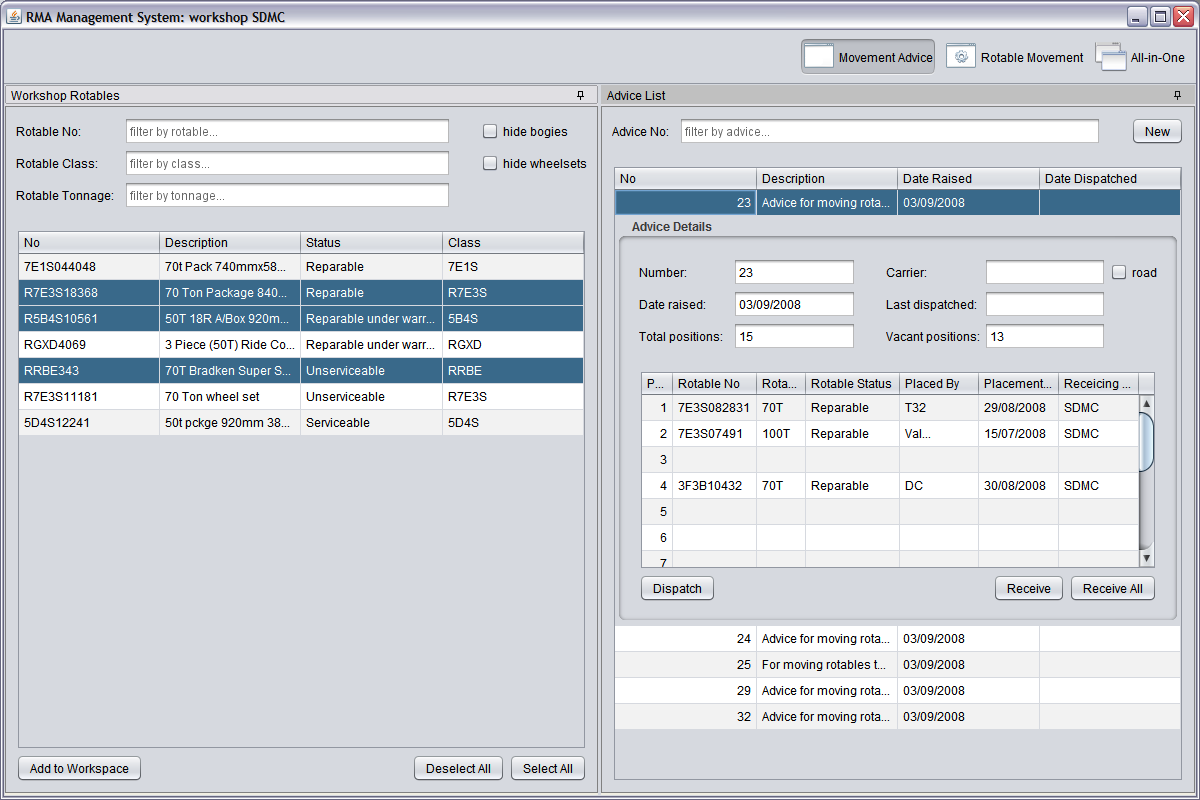
\includegraphics[scale=0.37]{chapters/02-user-interface/images/02-movement-advice-perspective-expanded.png}
\caption{Movement Advice }\label{fig:02-movement-advice-perspective-expanded}
\end{figure}

Both \emph{Workshop Rotables} and \emph{Advice List} provide a set of filtering criteria to effectively locate required information. Each filtering criterion is equipped with an autocompleter and performs data filtering on the fly while user is typing. These panels are dockable, which means the user can configure their sizes and positions. This information is automatically persisted -- the next time application is loaded, it will adhere to the stored user preferences. 
\\\\
A different perspective can be activated by using toggle buttons in the right side of the tool bar (the left side is reserved for other actions). \hyperref[fig:00-perspective-buttons]{Figure~\ref*{fig:00-perspective-buttons}} highlights this panel.

\begin{figure}[!h]
\centering
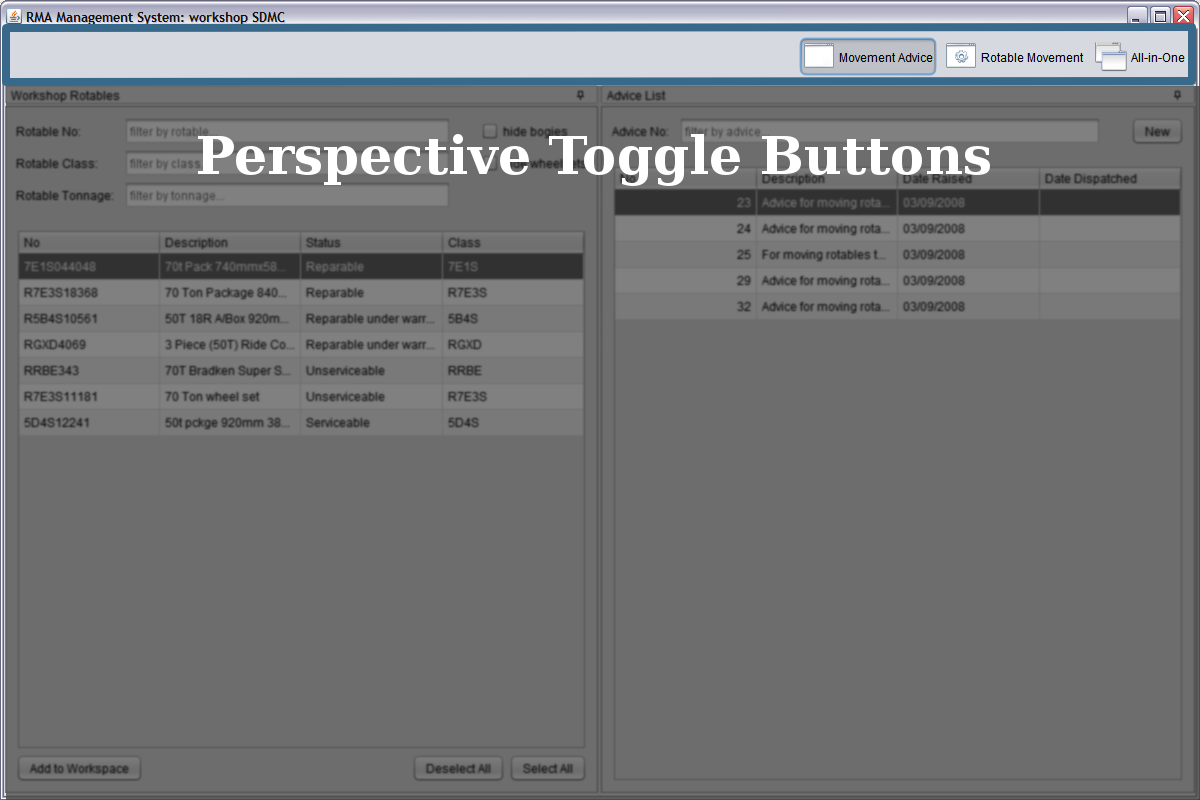
\includegraphics[scale=0.37]{chapters/02-user-interface/images/00-perspective-buttons.png}
\caption{Perspective Toggle Buttons}\label{fig:00-perspective-buttons}
\end{figure}

\clearpage

\subsection{Rotable Movement Perspective}
Clicking on the \emph{Rotable Movement} button in the tool bar activates a corresponding perspective, which is depicted in \hyperref[fig:04-rotable-movement-perspective-expanded]{Figure~\ref*{fig:03-rotable-movement-perspective}}.

\begin{figure}[!h]
\centering
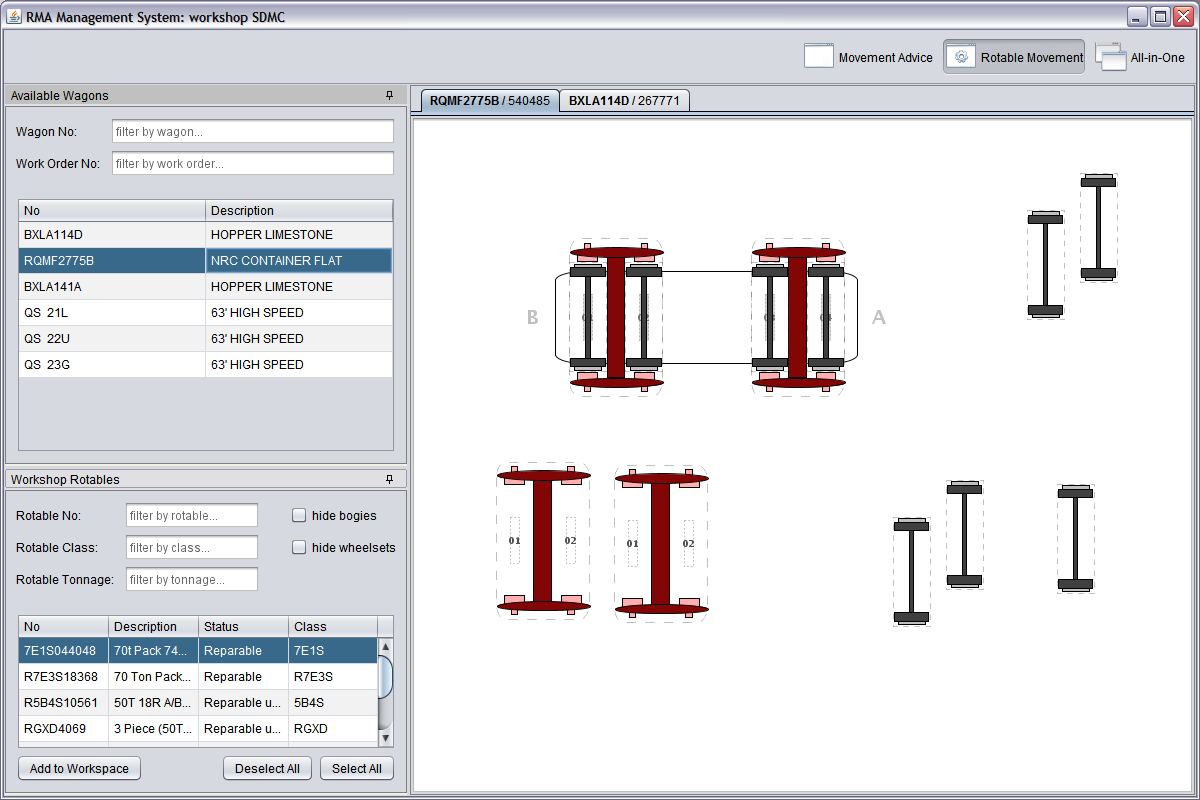
\includegraphics[scale=0.37]{chapters/02-user-interface/images/03-rotable-movement-perspective.png}
\caption{Rotable Movement Perspective}\label{fig:03-rotable-movement-perspective}
\end{figure}

This perspective is designed to address a narrow task of fitment/defitmet of rotables. It consists of a list of available wagons, rotables and a workspace area for interactive fitment/defitment operations.

When performing fitment/defitment, the user should know either the list (one and more) of wagons that need to be processed, or a list of work orders against those wagons. The \emph{Available Wagons} sub-panel provides an easy way to locate the required wagons. Only those wagons with active work orders for the specified workshop are displayed. The displayed list of wagons may still be too large to efficiently find the required ones. In order to overcome this, the sub-panel includes two filtering criteria -- by wagons and work orders. The filtering controls are autocompleters and support multiple values. So, the user can either type the required values or look'em up. When the user starts typing, the information in the grid is automatically filtered, so the user does not need to enter the whole wagon or work order number.

Our analysis of the current data suggests that there are situations where the wagons may have several fitment/defitment related active work orders in the same workshop. Therefore, when selecting a wagon to be added to the workspace it is necessary to specify one of the related work orders. The wagon grid provides the \emph{Wagon Details} view as a row expansion, which can be activated by selecting a row with a required wagon. Button \emph{Add to Workspace} should be used for adding wagons to the workspace as depicted in \hyperref[fig:04-rotable-movement-perspective-expanded]{Figure~\ref*{fig:04-rotable-movement-perspective-expanded}}. This button becomes enabled when one of the present work orders is selected. In case where there is only one work order this button is automatically enabled, saving the user the extra click.

\begin{figure}[!h]
\centering
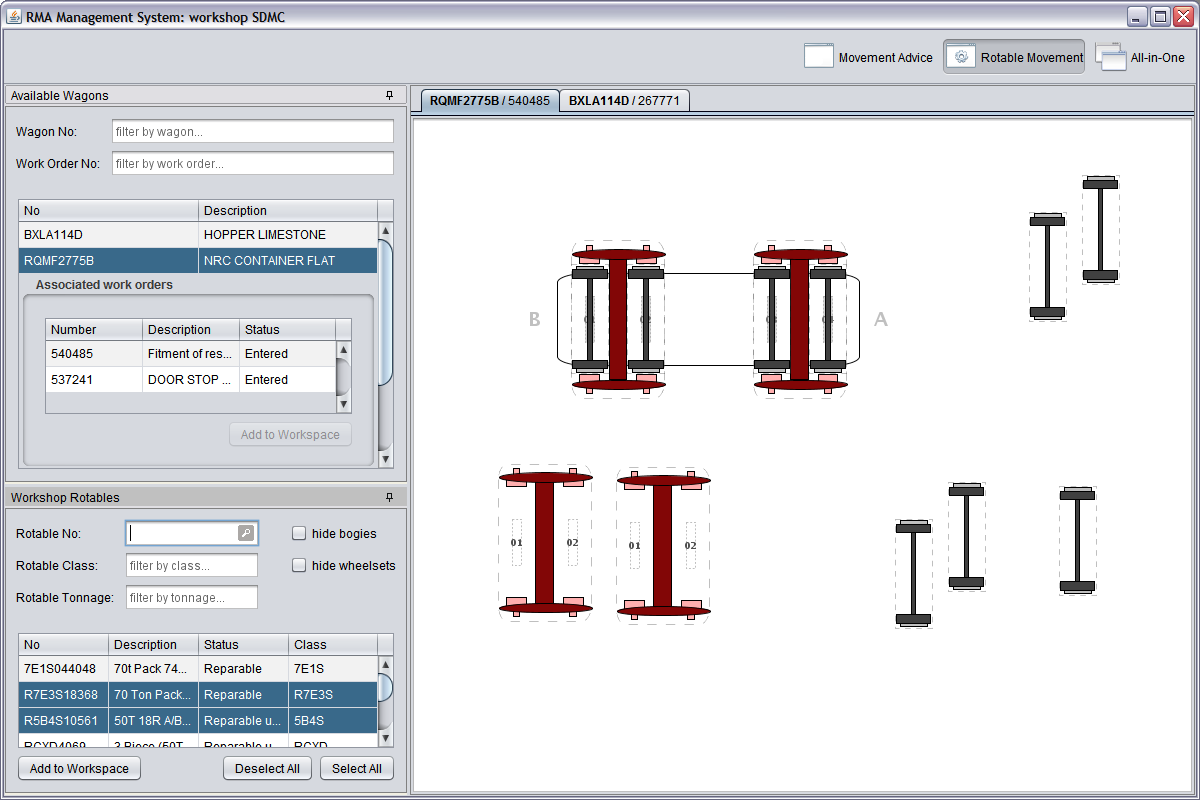
\includegraphics[scale=0.37]{chapters/02-user-interface/images/04-rotable-movement-perspective-expanded.png}
\caption{Wagon Details View}\label{fig:04-rotable-movement-perspective-expanded}
\end{figure}

\emph{Workshop Workspace} is an area where the user performs interactive rotable operations such as fitment, defitment and placement onto a movement advice. It is based on the iRMS functionality, but enhances it to the next level, striving to improve the user experience by simplifying the interaction. For example, the workspace features multiple rotable selection in the various operations (e.g. defitment).

Also, the iRMS user is often overloaded with information -- several widgets for different workshops, rotables available in the workshop etc. The workspace has been designed to contain only items requested by the user -- a wagon selected by the user and only those rotables from the workshop and/or movement advices that the user specifically added to the workspace.

The workspace supports tabsheets to enable the user to work on several wagons -- each in a separate tab. The tab caption provides information about the included wagon, as well as the related work order specified when adding wagon to the workspace.

Similar to other perspectives, the size an location of the sub-panels is user customizable. One additional feature not mentioned previously is the ability to make a tab-panel consisting of separate tabs for each of the sub-panels. \hyperref[fig:05-rotable-movement-perspective-with-tabs.png]{Figure~\ref*{fig:05-rotable-movement-perspective-with-tabs}} depicts a tabbed layout where tabs are located at the bottom of the left panel.

\begin{figure}[!h]
\centering
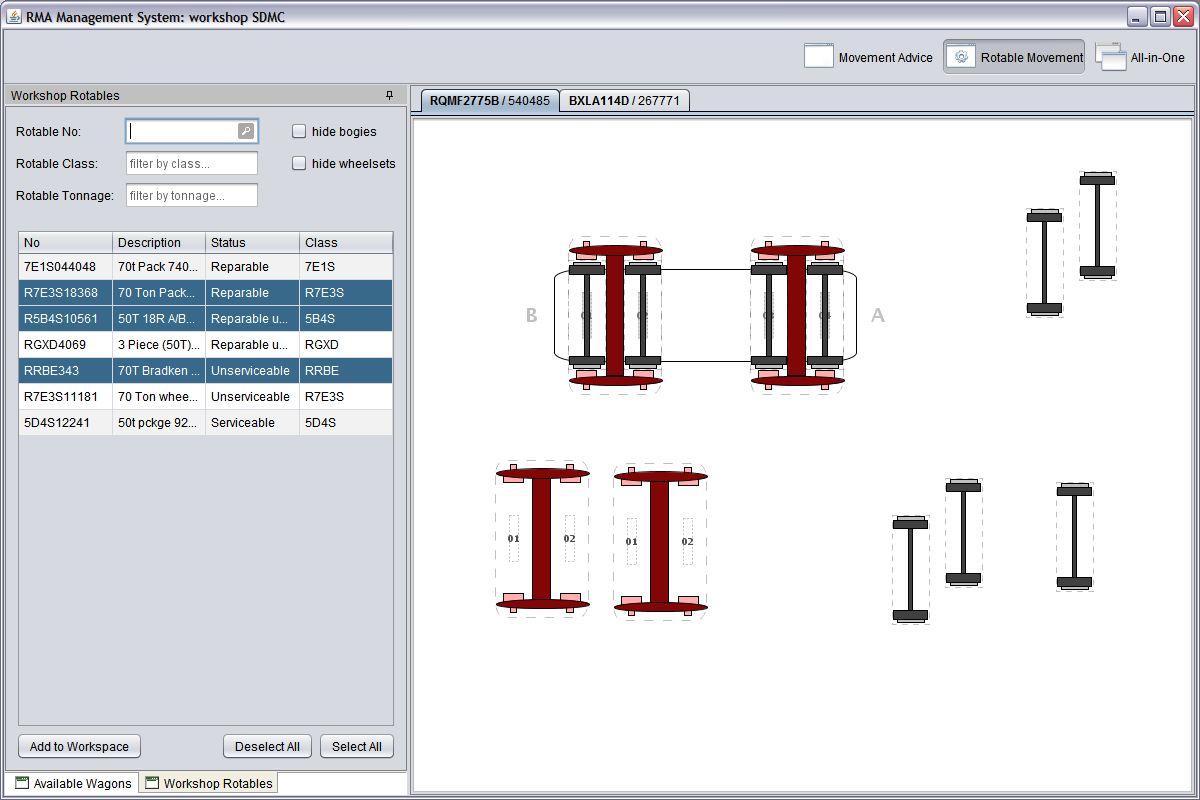
\includegraphics[scale=0.37]{chapters/02-user-interface/images/05-rotable-movement-perspective-with-tabs.png}
\caption{Tabbed Layout}\label{fig:05-rotable-movement-perspective-with-tabs}
\end{figure}
\clearpage

\subsection{All-in-One Perspective}
Two previous perspectives cater towards narrow activities -- movement advice processing and rotable fitment/defitment. However, these responsibilities can be combined. For example, user may want to defit rotables directly off the wagon onto a selected advice, or receive rotables for fitment directly into the workspace with preloaded wagon. For this purpose an advanced perspective \emph{All-in-One} was introduced, which combines controls from both previous perspectives.

The All-in-One perspective UI layout depicted in \hyperref[fig:06-all-in-one.png]{Figure~\ref*{fig:06-all-in-one}} is somewhat clattered. 

\begin{figure}[!h]
\centering
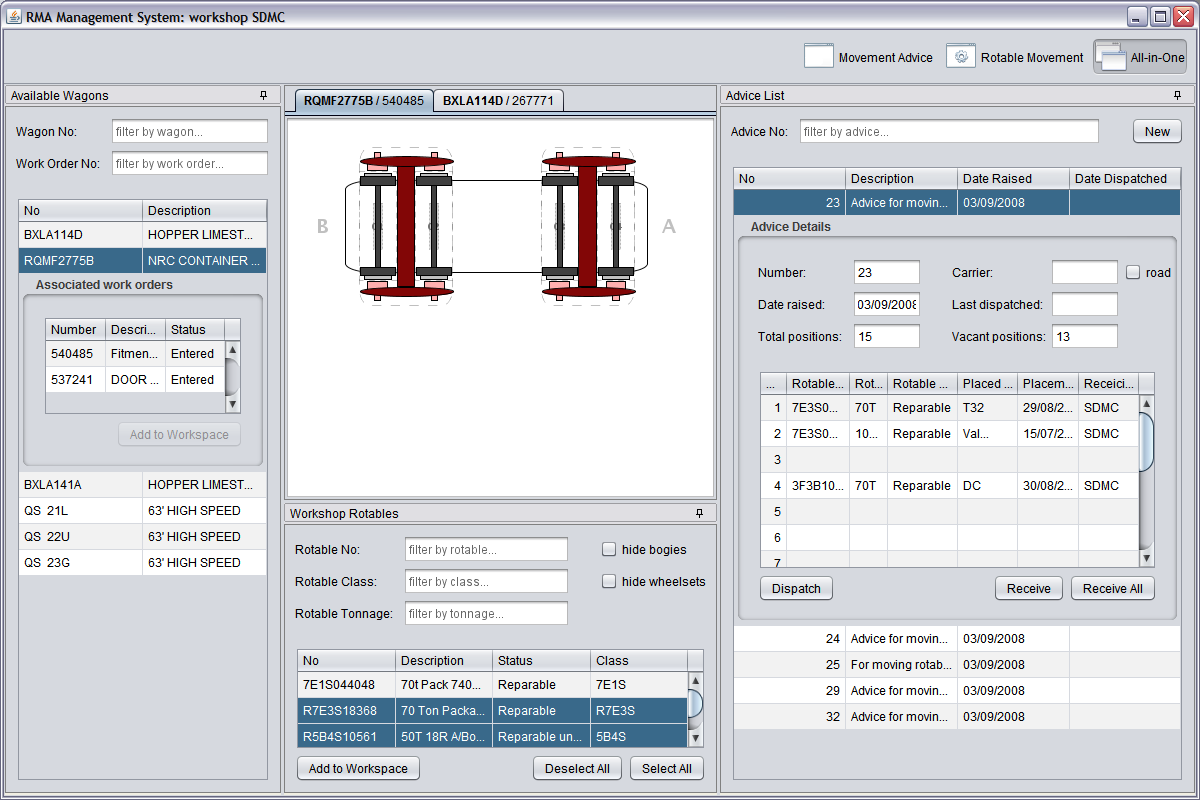
\includegraphics[scale=0.37]{chapters/02-user-interface/images/06-all-in-one.png}
\caption{All-in-One Perspective}\label{fig:06-all-in-one}
\end{figure}

However, the layout is customizable and user can do exactly what suits her/his needs and habits. As an example, \hyperref[fig:07-all-in-one-with-tabs]{Figure~\ref*{fig:07-all-in-one-with-tabs}} depicts the same All-in-One perspective, but in tab layout where Advice List, Available Wagons and Workshop Rotables are placed on separate tabs as part of the left panel.

\begin{figure}[!h]
\centering
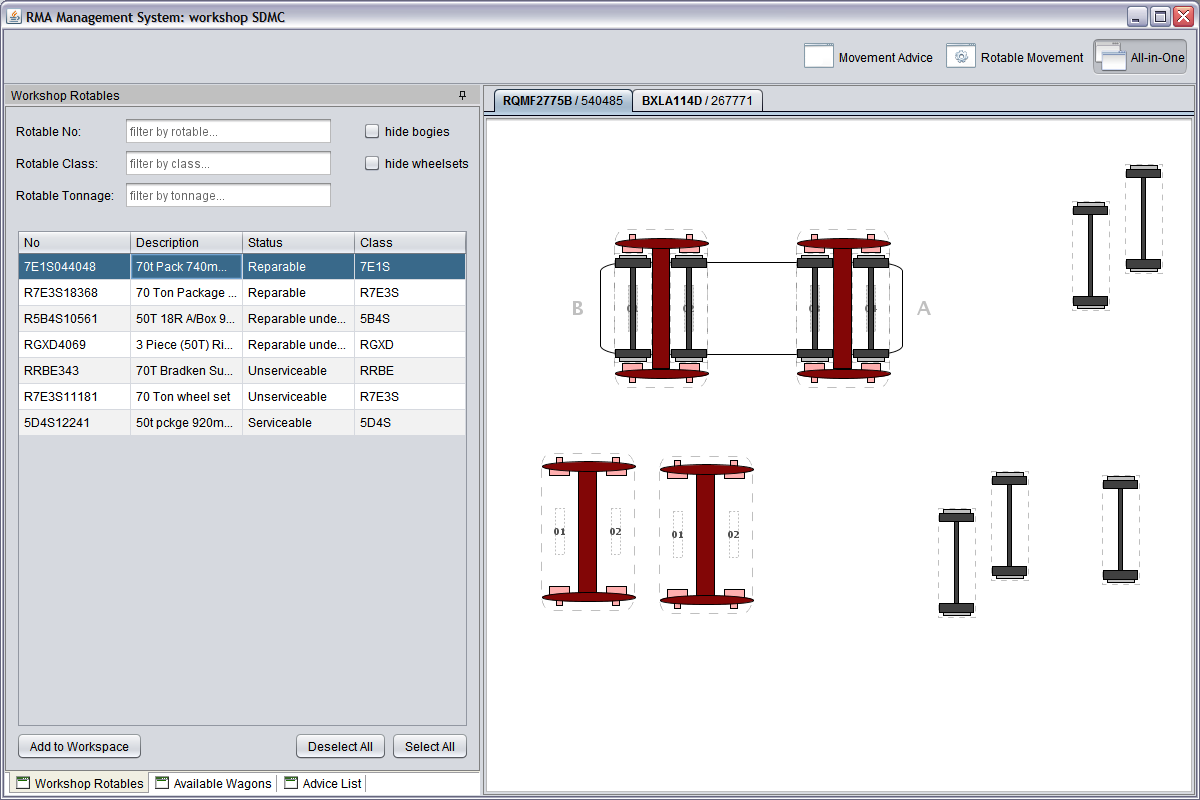
\includegraphics[scale=0.37]{chapters/02-user-interface/images/07-all-in-one-with-tabs.png}
\caption{All-in-One with tabs}\label{fig:07-all-in-one-with-tabs}
\end{figure}

Please refer \hyperref[fig:08-docking-tabsheets]{Figure~\ref*{fig:08-docking-tabsheets}} where these tabsheets are highlighted.

\begin{figure}[!h]
\centering
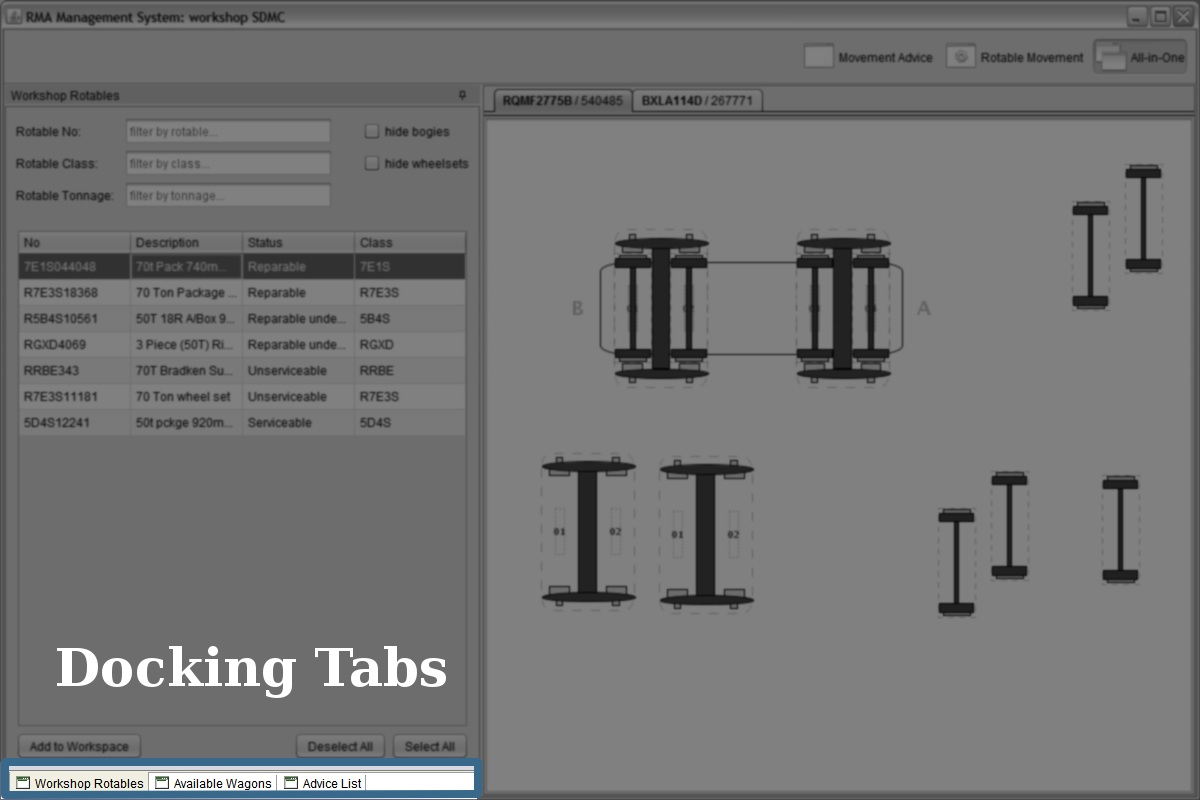
\includegraphics[scale=0.37]{chapters/02-user-interface/images/08-docking-tabsheets.png}
\caption{Highlighted Tabs}\label{fig:08-docking-tabsheets}
\end{figure}


\clearpage